\chapter{The Data} \label{ch:data}
\section{The data framework} \label{sec:framework}
The European framework for road accident data collection is called \ac{CADAS} \cite{cadas} and it established the rules that each country from the \ac{EU} should follow when recording accident data. It provides a simple accident data collection set and methodology containing the categories and attribute descriptions, composed of more than 100 rules that the records should be compliant with. 
In this way, by introducing a minimum set of standardised data elements common to all the European countries, harmonisation between accident data at national and \ac{EU} level can be achieved and, as a consequence, comparing road accident data from all \ac{EU} countries will be possible, giving place to interesting analyses. This would facilitate identifying and quantifying road safety issues throughout European roads, as well as evaluating the efficiency of the measures applied by each country. 
\\
\\
After analysing how each country in Europe was gathering their data, \ac{CADAS} was suggested as a minimum set of standardised data requirements, that will allow to compare road accident data from all European countries. Many of the countries had their own national data sets structure and definitions, making them not compatible or comparable among the different European countries. 
\\
\\
Using this framework proposed by the \ac{EC} will allow to transform the national data sets according to specific transformation rules, resulting in the fact that the CARE database will be formed with compatible data.
This is nowadays done at the \ac{EU} level, however, it could be a substantial basis for the expansion of other common data set to be used at global level allowing to compare and analyse accident data worldwide. 
The \ac{CADAS} guidelines will be followed later in Section \ref{sec:validation} to validate the format of the data and ensure its quality.
\\
\\
\ac{CADAS} structure:
the variables presented are divided into four categories, each of them identified by a unique letter that will allow to identify to which category each attribute belongs to. The categories and the letters used to recognize each category attribute are the following:
\begin{itemize}
    \item A: Accident related attributes
    \item R: Road related attributes
    \item U: Traffic Unit (vehicle and pedestrian) related attributes
    \item P: Person related attributes
\end{itemize}

In Figure \ref{fig:cadas}, it can be observed how the four tables are related, indicating the links between them and listing all the attributes for each of the categories. 

    
    \begin{figure}[H] 
    %\centering
    \captionsetup{justification=centering}
    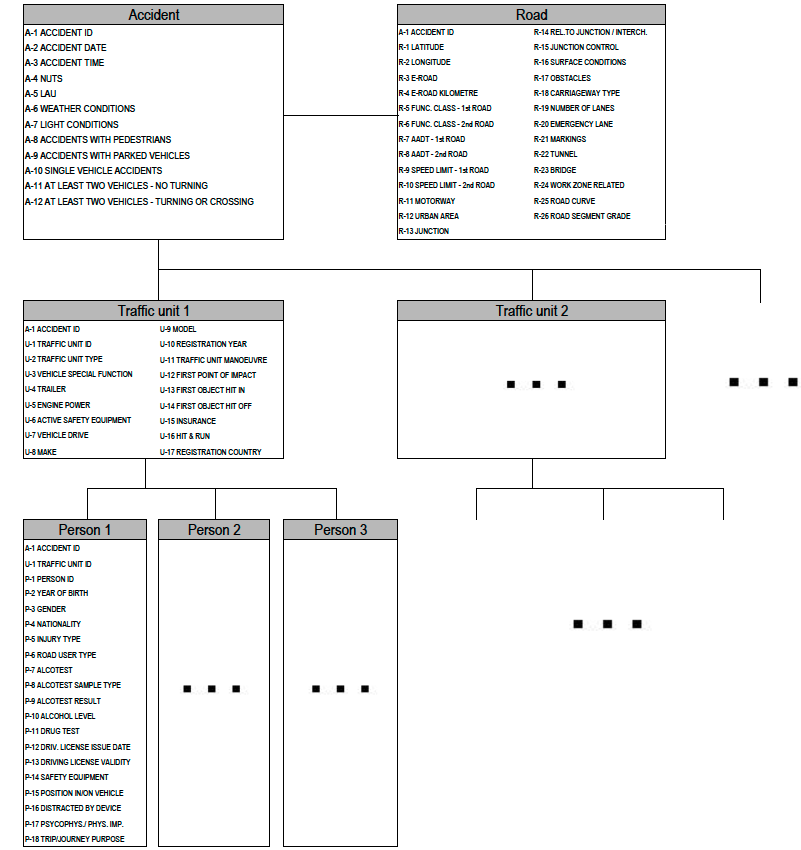
\includegraphics[width=1.17\textwidth]{Images/cadas.png}
    \caption[CADAS structure]{CADAS structure \parencite{cadas}}
    \label{fig:cadas}
    \vspace{-0.5em}
    \end{figure}
    
For each of the attributes included in \ac{CADAS}, the following information is given \cite{cadas}:
\begin{itemize}
    \item Variable label: the category identifier letter (A, R, U or P), its numbering and the attribute's name. 
    \item Variable definition and scope: description about the practicality of the attribute.
    \item List of values: the allowable values the attribute can take.
    \item Value labels: the code of the attribute followed by a number corresponding to each value and its name.
    \item Value definitions: the explanation of each value of the attribute.
    \item Data format: the format each attribute has to follow. 
\end{itemize}

Each country will generate four files (one for each category) after transforming their national data structure into the \ac{CADAS} structure. The files are named according to the normative as: XX\_ACCIDENT\_9999, XX\_ROAD\_9999, XX\_TRAFFIC\_UNIT\_9999, XX\_PERSON\_9999. Where "XX" represents the country code and "9999" has to be replaced by the corresponding year. For every year of data, a separate file must be created for each of the categories. 
\\
\\
The four main categories mentioned are described as follows: 
\begin{itemize}
    \item Accident information: this category contains basic information regarding the accident besides the type of conflict that it was and the direction of impact that crashing parties have encountered. 
    \item Road information: this category contains basic information regarding the road environment. When the accident occurs at a junction, part of this basic information is gathered for the two roads.
    \item Traffic unit information: this category contains basic information regarding the traffic unit (vehicles and pedestrians) that are affected in the road accident. 
    \item Person information: this category contains basic information regarding the road users participating in the road accident. This category attributes are recorded separately for each person involved in the accident.
\end{itemize}

\section{The provided data}
The data used in this research (provided by Sensmetry) consists of a relational database containing information about crashes on the roads in Lithuania for four years (2017-2020). It is composed of four different tables interrelated between them by an attribute key, namely, \textit{accident id}. The input to each table is a csv file, one for each table and for each year. Each table contains a different number of attributes describing the characteristics of the accident, road, person or traffic unit. The schema and template used for the tables in the database was designed by \ac{CADAS} as explained in Section \ref{sec:framework}.
\\
\\
The \ac{CADAS} structure gives a label based on the importance of the attributes, H for high priority and L for low. For the Lithuanian data, not all the fields listed in the \ac{CADAS} glossary were collected but all the ones with high priority label were. 
The tables for the analysed Lithuanian data are described as follows:
\begin{itemize}
    \item Accident Information: 12 attributes recording information about accident id, accident date and time, weather conditions, light conditions, etc. 
    \item Road Information: 25 attributes recording information about accident id, latitude, longitude, speed limit, etc.
    \item Person Information: 20 attributes recording information about accident id, the person's date of birth, gender, positive or negative alcohol test, driving license validity, etc.
    \item Traffic Unit Information: 18 attributes recording information about accident id, vehicle identification, type of vehicle, vehicle make, etc.
\end{itemize}

In total, the number of attributes to be processed is 65. Each attribute must follow the rules on \ac{CADAS} since each of them has unique characteristics. Their values and format need to be validated in order to ensure logical and syntactic conformity.  
The total number of accident records for the four years of available data is approximately 12000.
\\
\\
An exhaustive manual checking has been done to analyse, one by one, more than 100 rules that \ac{CADAS} determines, with the help of the glossary for transport statistics \cite{transport}. This required in many cases to get further clarification on specific terminologies from domain experts.
\\
\\
All those rules have been implemented in software unit tests and it has been used in data validation tests to check if the provided data is indeed compliant with \ac{CADAS}'s rules (see Section \ref{sec:validation}).
